\section{Implementation} \label{Implementation}

The starting point of our implementation is the Cothority Template \cite{Template}, which serves as an example on how to create a ByzCoin \cite{ByzCoin} blockchain service.\\
\newline
The main elements of the ByzCoin implementation are: \textbf{instructions} sent by the clients, \textbf{contracts} that define how the instructions are interpreted, a global state with \textbf{instances} which are tied to a contract and hold data, and \textbf{DARC structures} (explained bellow) for access control (Figure~\ref{ByzCoin simplified}).
\begin{figure}[H]
    \centering
    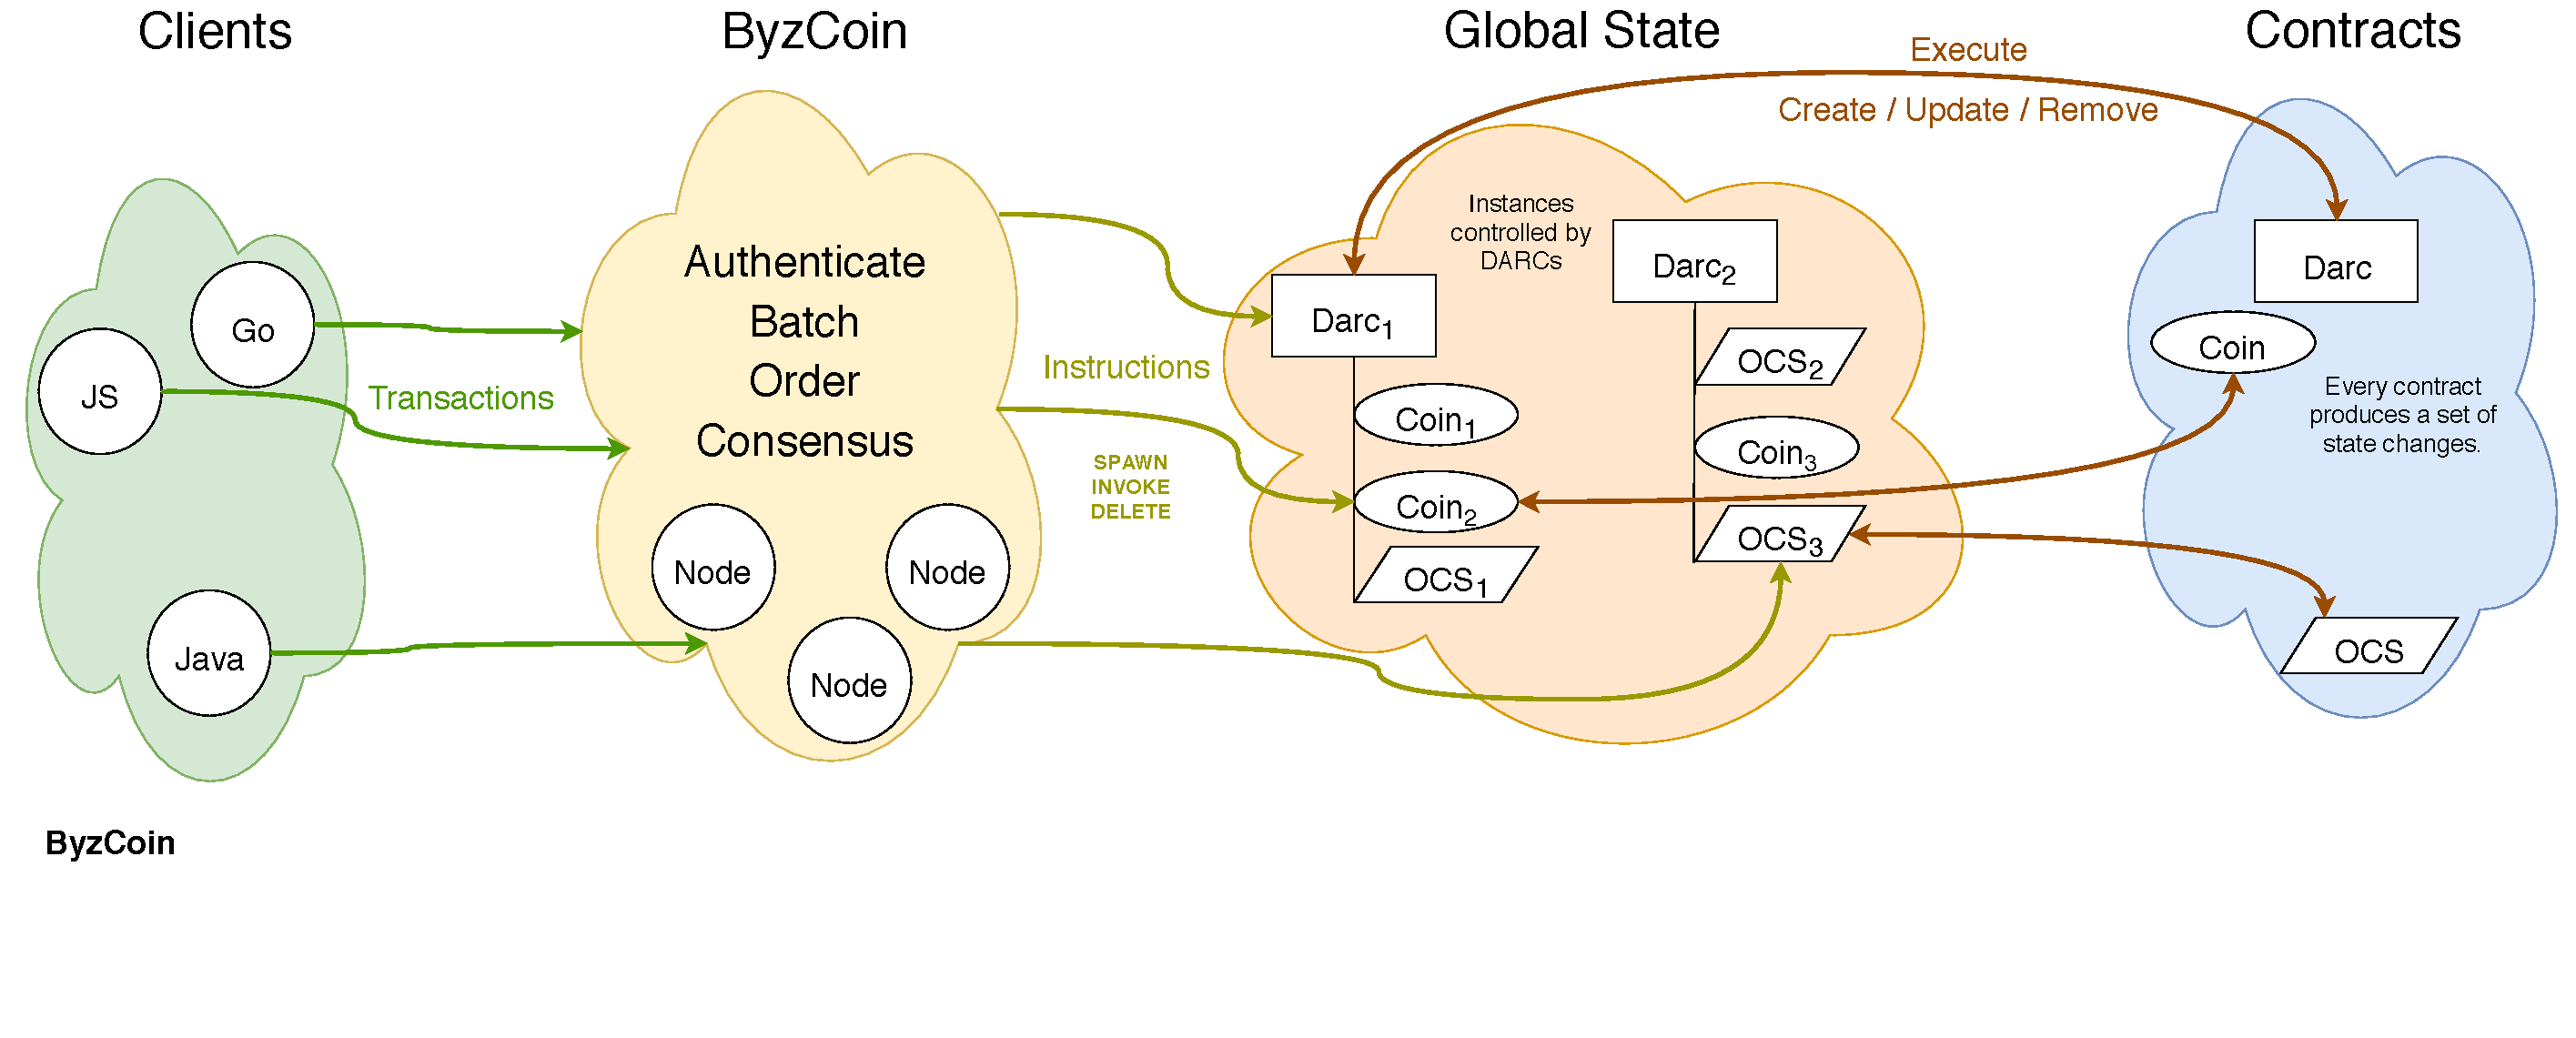
\includegraphics[width=1\textwidth]{Figures/ByzCoin_simplified.pdf}
    \vspace{-40pt}
    \caption{ByzCoin (Simplified version of \cite{ByzCoin Figure})}
    \label{ByzCoin simplified}
\end{figure}
\noindent
Every user instruction which is sent to the ByzCoin service can be one of: \textbf{spawn} for creation, \textbf{invoke} for update or \textbf{delete} for removal, and needs to have an existing instance as a target (Figure~\ref{ByzCoin simplified}). These instances maintain information about their unique \textbf{ID}, \textbf{version} which is the number updates, the \textbf{contract ID} tied to that particular instance, \textbf{data} to be interpreted by the contract and a \textbf{DARC ID} for access control \cite{Contracts}.\\
\newline
A detailed description of the ByzCoin implementation can be found on the DEDIS cohority git repository \cite{ByzCoin Impl}.

\subsection{Access Control with DARCs} \label{DARCs}

The management of access rights is handled by DARC structures (Distributed Access Right Controls) \cite{Darc}, which maintain a set of rules.
Every rule consists of an action name and an expression that contains identities allowed to execute that action.\\
\newline
DARCs can be updated by the identities specified in the \textbf{evolve} rule. There exists also a notion of delegating the permissions to another DARC, by specifying the DARC ID in the rule expression instead of an identity. This delegation plays an important part in the smooth transfer of car history ownership, that does not require an intervention by the administrator. On Figure ~\ref{DARCs Schema}, we can observe the schema of DARCs required for our project.\\
\newline
Due to the security guarantees of our system, only the administrator has the possibility to create new DARCs with the \textbf{spawn:darc} command.
Moreover, each participant (user) has a dedicated DARC, that will prevent losing his/her access rights upon losing credentials (private key), by including the administrator identity in the \textbf{evolve} rule.\\
\newline
Furthermore, for every enrolled car, there needs to exist a separate DARC for storing owner, writers (garage mechanics) and readers (potential buyers), as well as a car DARC with rules for: creating a car instance, adding reports, adding Calypso secrets and reading Calypso secrets.
\begin{figure}[H]
    \centering
    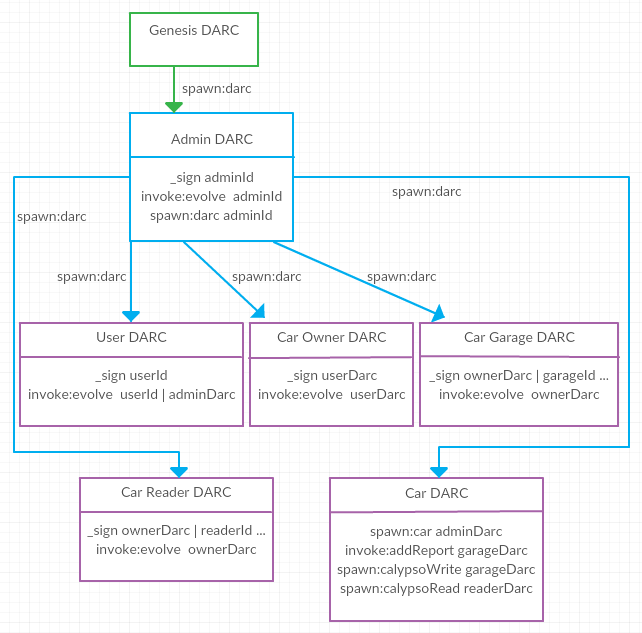
\includegraphics[width=1\textwidth]{Figures/DARCs_schema.png}
    \caption{DARCs Schema}
    \label{DARCs Schema}
\end{figure}
\noindent
\newline
Now that the DARC schema is determined, we can proceed to creating the digital contracts that define what happens in the global state once some particular command is invoked.

\subsection{ByzCoin Contracts}

The term smart contract is being used for digitally enforcing specific performance. ByzCoin contracts resemble the Ethereum smart contracts \cite{Ethereum} with the difference that they are precompiled and every node needs to have the same version in the interest of achieving consensus \cite{Contracts}.\\
\newline
Digital contracts \cite{Contracts} regarding the ByzCoin configuration, the access control and the Calypso functionality are predefined and take part of the cothority project \cite{Cothority}.
What is missing for our service is an additional contract related to the car instances, which had to be first designed and then registered with ByzCoin.\\
\newline
Within this car contract, we define methods for the \textbf{spawn} and the \textbf{invoke} type of instructions which create or update car instances accordingly (Section ~\ref{Implementation}). A method for the \textbf{delete} instruction is intentionally omitted in the car contract as we wouldn't like any vehicle's maintenance history to be erased.\\
\newline
Before creating a new car instance in the global state, we firstly check whether the data corresponds to a car object with a string of vehicle identification number (VIN) and an empty list of reports (Table~\ref{Data Structures}). If the verification is correct, a new state change is being made. The command for this instruction is named \textbf{spawn:car}.\\
\newline
When updating a car instance, a report is being added to the list of reports about that particular car. Every report consists of a string representing the ID of the garage mechanic that submitted the report, the date of the maintenance check and a calypso write instance that keeps secret data like for example: mileage, repairs, warranty, etc (Table~\ref{Data Structures}). The command for this update instruction is named \textbf{invoke:addReport}.
\begin{table}[h!]
    \centering
 \begin{tabular}{|c | c |c|} 
 \hline
 SecretData & Report & Car \\ [0.5ex] 
 \hline
 string ECOScore & string Date  & string VIN \\ 
 \hline
 string Mileage & string GarageID & [ ]Report Reports \\
 \hline
 boolean Warranty & [ ]byte WriteInstanceID &  \\
 \hline
 string CheckNote & & \\ [0.5ex]
 \hline
\end{tabular}
\caption{Data Structures}
\label{Data Structures}
\end{table}
\newline
With this being specified, the car contract is ready to be registered.




\subsection{Calypso Interaction}

Before we dive into the usage of Calypso in our system, let us first take a look at how Calypso is actually implemented \cite{Calypso Implementation}.
\newline
As presented in the section \ref{ByzCoin Background}, Calypso requires two collective authorities:
\begin{itemize}
    \item Access Control Cothority
    \item Secret Management Cothority
\end{itemize}
In our implementation, we use the same nodes to constitute both access control and secret management cothorities.\\
\newline
\begin{figure}[H]
    \centering
    \includegraphics[width=1\textwidth]{Figures/CalypsoByzCoin.png}
    \caption{Calypso \cite{Calypso Implementation}}
    \label{Calypso}
\end{figure}
\noindent
As mentioned before, at the initialization of the blockchain service, the administrator needs to generate a distributed key pair for the secret-management cothority (Figure~\ref{Calypso} Step 1). Every writer in the system (garage mechanic from Figure~\ref{Use Case Diagram}) encrypts the symmetric key of his encoded secret with this collective public key.\\
\newline
Furthermore, the access control cothority runs the ByzCoin protocol and also maintains calypsoRead and calypsoWrite contracts. Thus, readers (potential buyers from Figure~\ref{Use Case Diagram}) and writers (garage mechanics) can use it for spawning read and write instances accordingly, as well as DARCs for access control (Figure~\ref{Calypso} Steps 2, 3, 4 and 5).\\
\newline
Finally, having the Read and Write Instance IDs, the reader (potential buyer) is able to request the secret-management cothority to re-encrypt the symmetric key used to encrypt the secret by the garage mechanic, with the public key of the reader in order to be able to decode the secret data (Figure~\ref{Calypso} Step 6).

With this being explained, we can continue with the inclusion of Calypso into our project.\\
\newline
The car ByzCoin contract enables creation of car instances. Once they exist on the blockchain, the authorized garage mechanics are able to add reports about them. 
\newline
Adding such maintenance reports consists of two steps, i.e. two different instructions (Figure ~\ref{Add Reports and Read History}):
\begin{enumerate}
  \item Spawning a Calypso Write Instance that holds the private data (encrypted using symmetric encryption)
  \item Updating the Car Instance by appending a new report to the list
\end{enumerate}
In order to read the car "biography", a potential buyer needs to go through the blockchain and find the block where the car instance is stored. This process is much faster when using the DEDIS skipchains \cite{Chainiac}, thanks to the long-distance links. The following steps are required for the potential buyer when reading a maintenance history:
\begin{enumerate}
  \item Obtaining the car data (VIN and list of reports)
  \item Spawning a new Calypso Read Instance, by using the Write Instance ID from the report
  \item Requesting the re-encryption key from the Calypso Secret Management Cothority, by providing the Read and Write Instances
  \item Receiving the re-encryption key and decoding it by using his/her private key
  \item Decrypting the secret
\end{enumerate}
For each report, steps from 2 to 5 need to be repeated.\\
\newline
Thanks to Calypso, it is cryptographically hard to learn any information about the maintenance histories of the cars on the blockchain, unless having the permission to do so.

\begin{figure}[H]
    \centering
    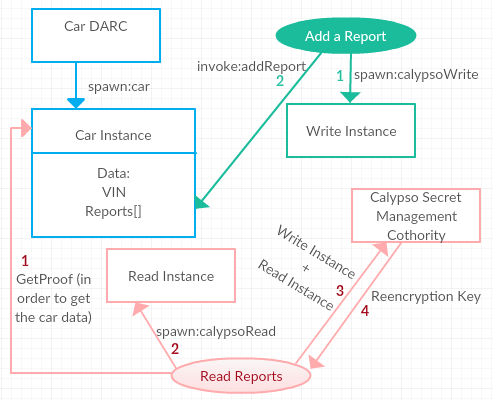
\includegraphics[width=1\textwidth]{Figures/add_read_reports.png}
    \caption{Add Reports and Read History}
    \label{Add Reports and Read History}
\end{figure}

 

\subsection{Client Application}
Having the car contract defined, together with the DARC structure for the system, we were able to create unit and integration tests in order to make sure everything works as expected (including the interaction with Calypso).
\newline
Once these tests passed and proved the correct functionality of the system, we were confident about moving forward with developing a user friendly interface for communication between the end users and the distributed ledger.
\\
\newline
In order to implement a desktop application, we decided to use the JavaFX software platform. To this end, we needed to use protocol buffers (mechanism for serializing structured data\cite{Protocol Buffers}) for a conversion from "Go" to "Java", and we also repeated our unit and integration tests, but this time in the Java programming language.\\
\newline
We designed the desktop application in such a way that the necessary configuration data, as well as the private credentials are stored locally in JSON format.
\begin{figure}[H]
    \centering
    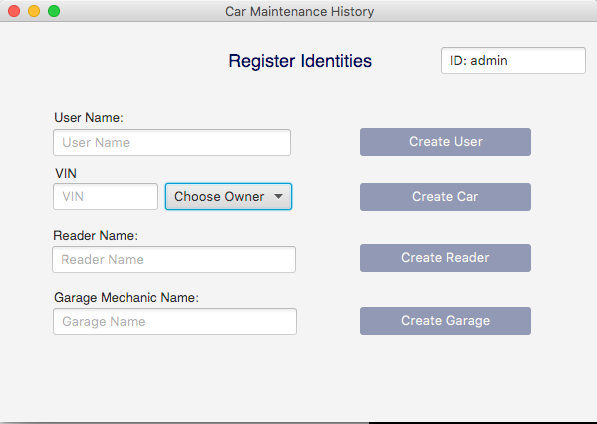
\includegraphics[width=1\textwidth]{Figures/DesktopApp/adminScreen.png}
    \caption{Admin Screen}
    \label{Admin Screen}
\end{figure}
\noindent
On the home screen, for demo purposes, it is possible to choose the identity from all enrolled participant and the administrator. The administrator is able to further register new cars, as well as new members (Figure ~\ref{Admin Screen}). As a reminder from chapter 4, it means adding all necessary DARCs for access control in the global state. The new members can either be: users with potential to become car owners, readers with the possibility to request car "biographies" or garage mechanics intended to add maintenance reports.\\
\newline
A car owner can use the desktop application to grant and remove access rights to potential buyers and garage mechanics for every vehicle he/she possesses (Figure ~\ref{Car Owner Screen}). It is also possible, on the same screen, to transfer the ownership of the selected car. Each one of these options updates the responsible DARC with the \textbf{invoke:evolve} command.\\
\newline
Once a garage mechanic has been granted a write permission, he/she is able to generate review about the current state of the checked vehicle and place it in a blockchain transaction (Figure ~\ref{Garage Mechanic Screen}).
\newline
Currently, a report consists of data about the mileage, warranty, score of how well the vehicle has been driven and a check-up note, but it is always possible to add additional parameters like for example the number of accidents.
\begin{figure}[H]
    \centering
    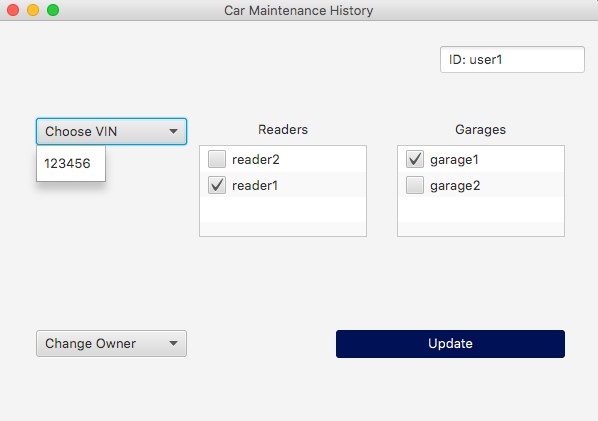
\includegraphics[width=1\textwidth]{Figures/DesktopApp/userScreen.png}
    \vspace{-15pt}
    \caption{Car Owner Screen}
    \label{Car Owner Screen}
\end{figure}

\begin{figure}[H]
    \centering
    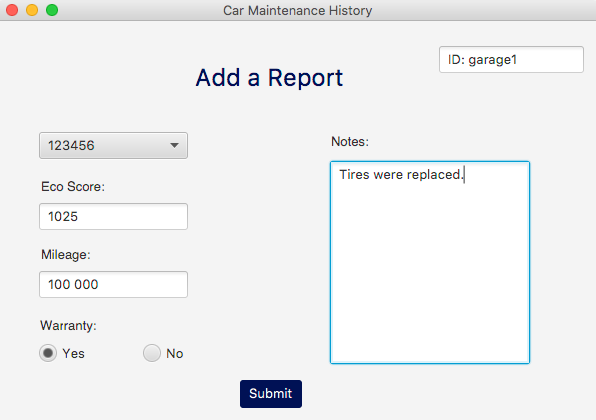
\includegraphics[width=1\textwidth]{Figures/DesktopApp/addReportScreen.png}
    \vspace{-15pt}
    \caption{Garage Mechanic Screen}
    \label{Garage Mechanic Screen}
\end{figure}
\noindent
When a potential buyer enters the application, it is possible to request the maintenance history of the chosen car (Figure ~\ref{Reader Screen}). If he/she is not allowed to access it, the application shows an error. 
\begin{figure}[H]
    \centering
    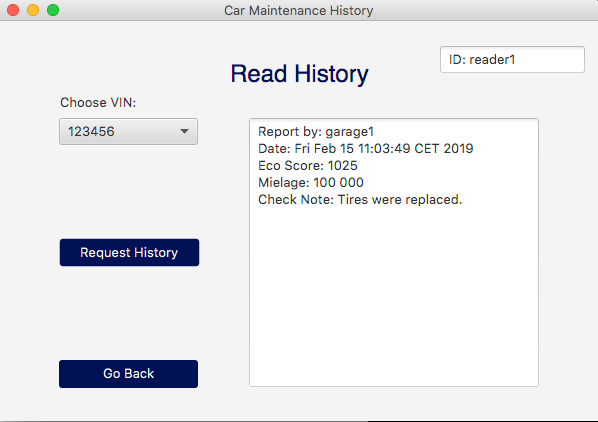
\includegraphics[width=1\textwidth]{Figures/DesktopApp/readHistoryScreen.png}
    \vspace{-15pt}
    \caption{Potential Buyer Screen}
    \label{Reader Screen}
\end{figure}


\subsection{Integration with the ByzCoin Skipchain Explorer}
Many blockchain implementations include a tool that enables users know detailed information about which transactions are taking part of a particular block.\\
\newline
For our project, we are connecting the car ByzCoin blockchain to a SkipChain Explorer \cite{Skipchain Explorer}, that has been developed as a student project in the DEDIS Laboratory at EPFL.\\
\newline
On Figure~\ref{SkipChain Explorer} we can see the current interface of the SkipChain Explorer, which contains the block number, transactions with instructions (\textbf{addReport} in this case), status (accepted or rejected), as well as signatures.\\ 
\newline
It is also possible to visualize the skipchain as a graph made of blocks, and load information only about the blocks we are interested in.
\begin{figure}[H]
    \centering
    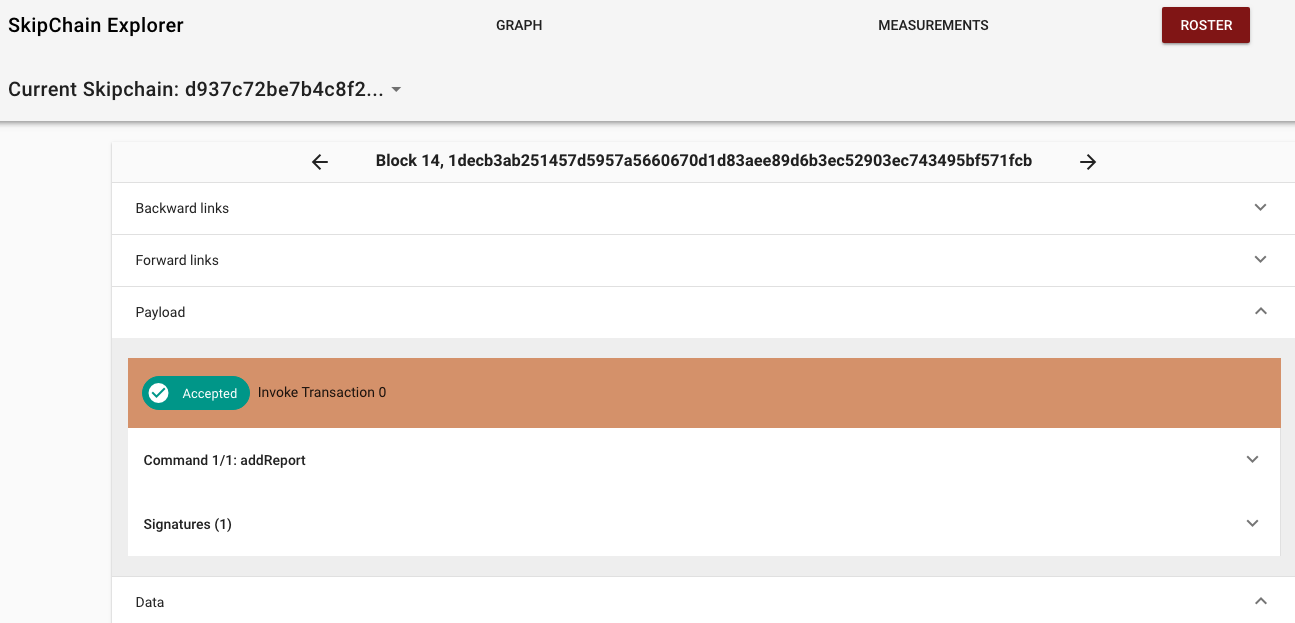
\includegraphics[width=1\textwidth]{Figures/SkipChain_Explorer.png}
    \caption{SkipChain Explorer}
    \label{SkipChain Explorer}
\end{figure}
\newline
\noindent
After being confident about the correctness of our implementation, we were able to proceed with evaluating our work in a more realistic setup (larger networks).